\documentclass[english]{article}
\usepackage[T1]{fontenc}
\usepackage[latin9]{inputenc}
\usepackage{geometry}
\geometry{verbose,tmargin=1cm,bmargin=1cm,lmargin=1in,rmargin=1in,headheight=1cm,headsep=1cm,footskip=1cm}
\pagestyle{empty}
\setcounter{secnumdepth}{2}
\setcounter{tocdepth}{2}
\usepackage{amstext}
\usepackage{graphicx}
\usepackage{babel}
\begin{document}
\begin{center}

{\huge Instructions: The Rook's Walk Puzzle}{\huge \par}

\end{center}\rule[0.5ex]{1\columnwidth}{1pt}

\noindent One pleasant, breezy afternoon, the Rook takes a walk though
its fine castle garden in the following way.
\begin{enumerate}
\item The Rook starts somewhere in the garden and moves $N$ squares in some direction (North, South, East, West).
\item Upon arriving at the $N^{\text{th}}$ square, the Rook writes the
number $N$ in the dirt and then chooses a new \textbf{different}
direction to travel in next.
\item The Rook repeats this until arriving back where it started in such a way that there are \textbf{no duplicate numbers} written in any given row or col of the garden. 
\end{enumerate}
Provided the sums of the numbers along each row and col of the garden and a few of the specific numbers used, can you determine the course the Rook took?  Hint: The rook cannot pass though any black spaces (marked -1 in my current output) and passes through any blank white spaces at least once (marked 0 in my current output).  

%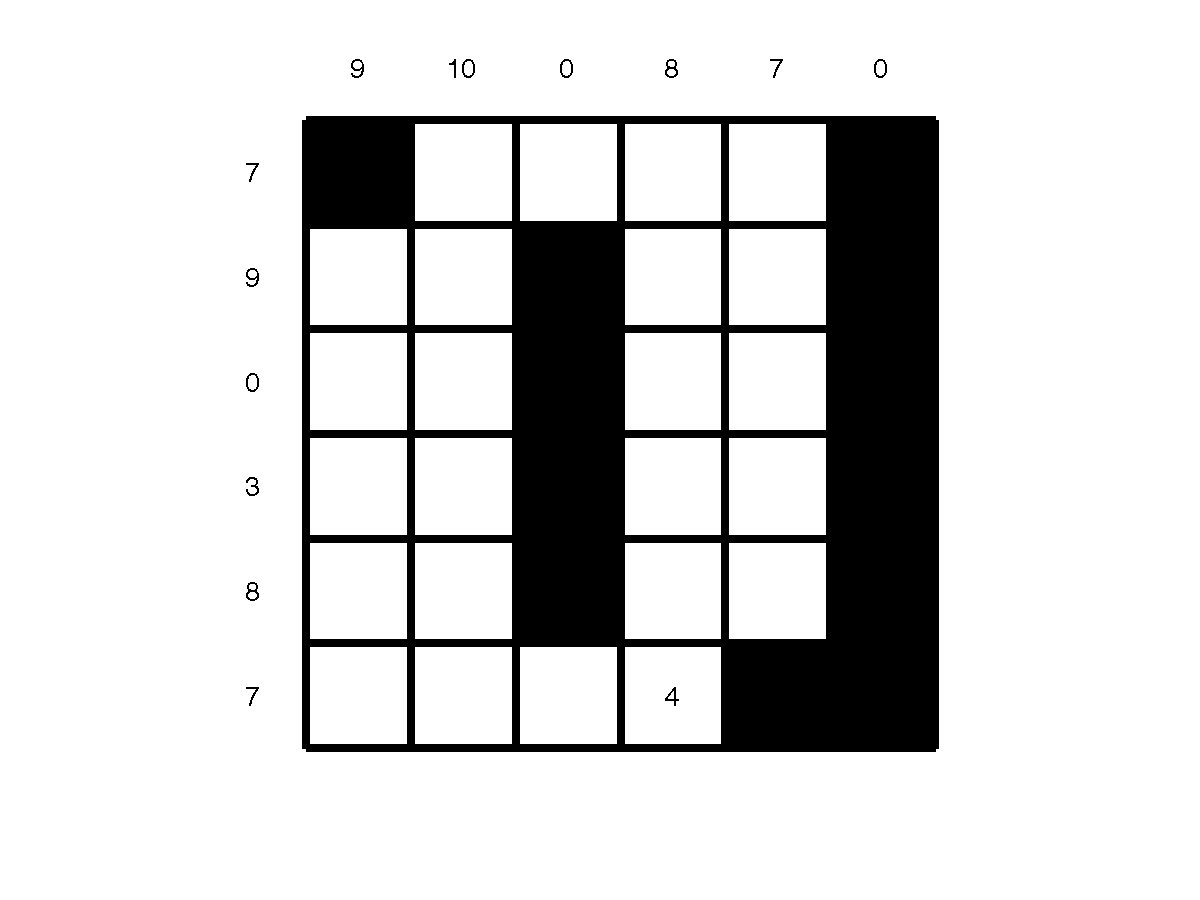
\includegraphics[scale=0.4]{medium}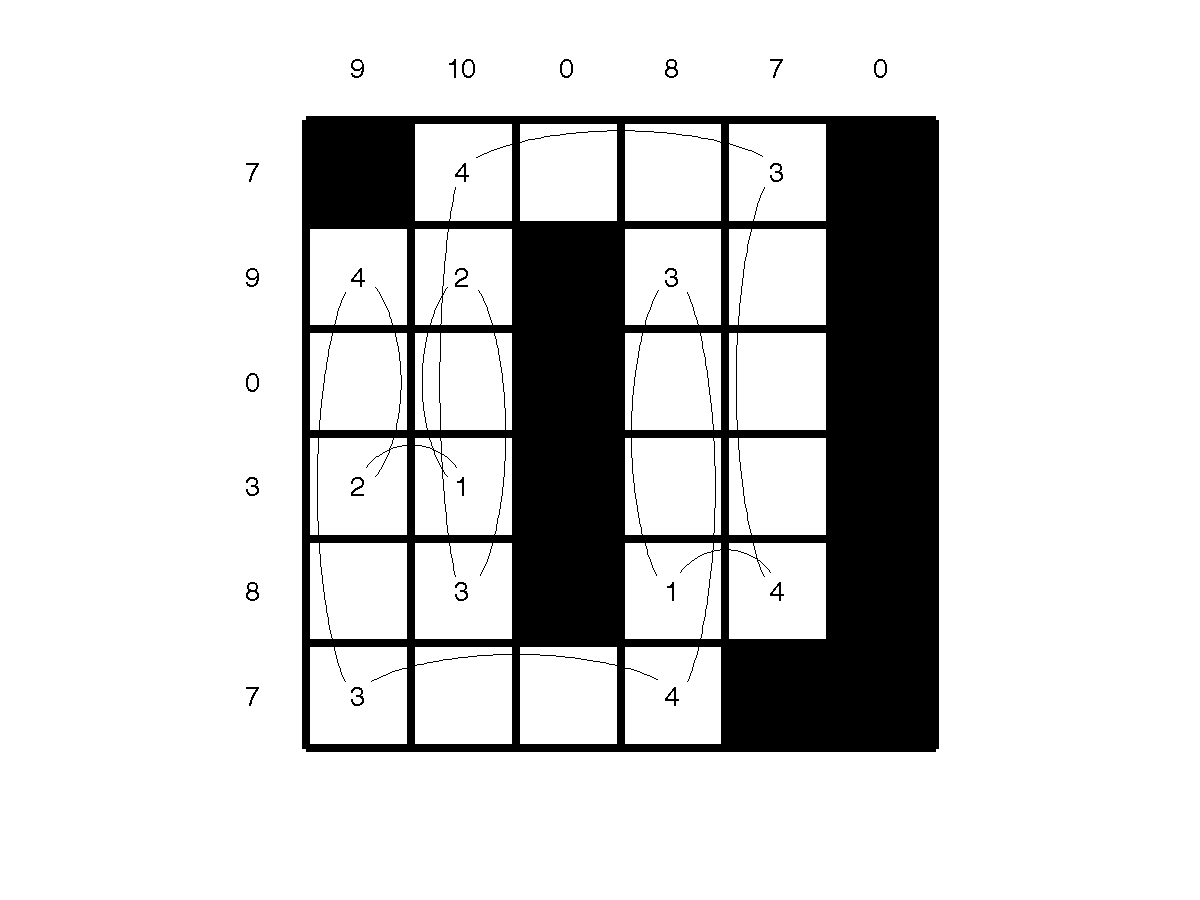
\includegraphics[scale=0.4]{mediumsoln}
\end{document}
